\appendix
\addtocontents{toc}{\protect\renewcommand*{\protect\chaptername}{PHỤ LỤC}}
\chapter{MÃ NGUỒN VÀ TÁI LẬP}
\label{app:code}

\section{Tổ chức mã nguồn}
Mã nguồn được công bố tại \url{https://github.com/HoanBuCon/UTCI-Vision}. Thư viện chính \texttt{utci\_vision} chứa từng khâu của pipeline dưới dạng một mô-đun; các script chạy thí nghiệm và công cụ dữ liệu nằm trong \texttt{scripts/} (Bảng~\ref{tab:code_structure}). Dữ liệu, trọng số và video không được đưa vào kho mã; chúng được tạo lại hoặc tải theo hướng dẫn ở Mục~\ref{sec:reproduce}.

\begin{table}[H]
\centering
\caption{Cấu trúc mã nguồn}
\label{tab:code_structure}
\footnotesize
\begin{tabularx}{\textwidth}{|>{\ttfamily\raggedright\arraybackslash}p{6.1cm}|X|}
\toprule
\textbf{\normalfont Tệp / thư mục} & \textbf{Chức năng} \\
\midrule
src/utci\_vision/enhance.py & [CV] Đánh giá chất lượng; gamma tự động, CLAHE kênh L, lọc song phương \\ \hline
src/utci\_vision/detector.py & [DL] YOLO11s: suy luận, FP16, cắt ô chồng lấn \\ \hline
src/utci\_vision/tracking.py & [CV] Kalman + Hungarian theo IoU, bỏ phiếu nhãn theo vết \\ \hline
src/utci\_vision/verifier.py & [CV + DL] Đặc trưng HSV, hình học, Hu, HOG + ngữ cảnh YOLO $\rightarrow$ LightGBM \\ \hline
src/utci\_vision/ocr.py & [CV + DL] Cắt vùng số, dòng chữ, biển phụ; VietOCR; regex + từ điển \\ \hline
src/utci\_vision/traditional.py & [CV] Pipeline đối chứng: HSV $\rightarrow$ hình thái học $\rightarrow$ hình dạng $\rightarrow$ HOG + màu $\rightarrow$ SVM \\ \hline
src/utci\_vision/pipeline.py & Ghép các khâu theo cấu hình; dùng chung cho API, video, webcam, đánh giá \\ \hline
src/utci\_vision/api/ & FastAPI: ảnh, video nền, WebSocket, so sánh, ảnh mẫu \\ \hline
src/utci\_vision/evaluation/ & Ghép dự đoán, mAP, bootstrap, Wilson, ảnh xấu giả lập \\ \hline
configs/*.yaml & Cấu hình lớp (QCVN), dữ liệu, YOLO, pipeline, bộ xác minh, OCR, pipeline truyền thống \\ \hline
scripts/data.py, eda.py & Kiểm tra, tìm ảnh gần trùng, chia theo cụm, đóng gói; phân tích dữ liệu \\ \hline
scripts/analyze\_run.py & Đánh giá S1: CI bootstrap, theo kích thước, lớp, mức tương đồng \\ \hline
scripts/verifier\_feasibility.py & T0, T1 \\ \hline
scripts/compare\_traditional\_dl.py & E8 \\ \hline
scripts/enhance\_robustness.py & T4 \\ \hline
scripts/evaluate.py & E1, E2 (\texttt{--ablation}), E4 (\texttt{--degrade dark}), T3 (\texttt{small}), tốc độ \\ \hline
scripts/train\_hog\_svm.py, fit\_verifier.py & Huấn luyện SVM của pipeline đối chứng và bộ xác minh \\ \hline
notebooks/train/ & Ba notebook tinh chỉnh YOLO11 (máy cá nhân, Colab, Kaggle) \\ \hline
web/ & Giao diện React + TypeScript \\ \hline
experiments/registry.csv & Sổ đăng ký mọi lần chạy và đánh giá \\ \hline
tests/ & Kiểm thử đơn vị và kiểm thử hợp đồng API (pytest) \\
\bottomrule
\end{tabularx}
\end{table}

\section{Cài đặt lõi}
Đoạn mã~\ref{lst:enhance} là quy tắc chọn phép tăng cường và gamma tự động (Mục~\ref{sec:enhance}); Đoạn mã~\ref{lst:candidates} là phần lọc hình dạng của pipeline đối chứng (Mục~\ref{sec:cv_pipeline}).

\begin{lstlisting}[language=Python, caption={Chọn phép tăng cường và gamma tự động (rút gọn từ \texttt{enhance.py}).}, label={lst:enhance}]
def needed_ops(q, cfg):
    ops = set()
    if q.mean_v < cfg["dark_mean_v"]:            # 0.30
        ops |= {"gamma", "clahe"}
    if q.std_l < cfg["low_contrast_std_l"]:      # 0.13
        ops.add("clahe")
    if q.laplacian_var > cfg["noisy_laplacian"]: # 4000
        ops.add("denoise")
    return ops

def auto_gamma(img, target=0.5, lo=0.4, hi=3.0):
    mean = np.clip(cv2.cvtColor(img, cv2.COLOR_BGR2HSV)[..., 2].mean() / 255, 1e-3, 0.999)
    return float(np.clip(np.log(mean) / np.log(target), lo, hi))   # out = in^(1/gamma)
\end{lstlisting}

\begin{lstlisting}[language=Python, caption={Lọc ứng viên theo hình dạng (rút gọn từ \texttt{traditional.py}).}, label={lst:candidates}]
hull = cv2.convexHull(c)
hull_circ = 4 * np.pi * cv2.contourArea(hull) / cv2.arcLength(hull, True) ** 2
if 0.6 <= aspect <= 1.6 and hull_circ >= 0.75:
    shape = "circle"        # red ring of prohibitory signs is hollow -> use convex hull
elif color in ("red", "yellow") and vertices == 3 and 0.7 <= aspect <= 1.5 and solidity > 0.6:
    shape = "triangle"
elif color == "blue" and 4 <= vertices <= 6 and 0.5 <= aspect <= 3.0 and solidity > 0.8:
    shape = "rectangle"
\end{lstlisting}

\section{Hướng dẫn tái lập}
\label{sec:reproduce}

\paragraph{Cài đặt.} Cần Python 3.11 trở lên, Node.js và (tuỳ chọn) GPU NVIDIA. Các lệnh chính:
\begin{lstlisting}[language=bash]
git clone https://github.com/HoanBuCon/UTCI-Vision.git && cd UTCI-Vision
make env && make venv          # .env (custom ports) and virtual environment
# install torch matching the GPU / CPU, then:
make install && make check-env
\end{lstlisting}

\paragraph{Dữ liệu và trọng số.} Tải bộ dữ liệu gốc từ Roboflow~\cite{roboflow_dataset} vào \texttt{dataset/raw}, rồi tạo lại \texttt{processed/v1} bằng \texttt{python scripts/data.py audit --dedup} và \texttt{python scripts/data.py split}; mã băm SHA-256 của gói dữ liệu được ghi trong hồ sơ dữ liệu. Trọng số YOLO11s được nhập bằng \texttt{scripts/import\_run.py --promote}; SVM của pipeline đối chứng và bộ xác minh được tạo lại bằng \texttt{scripts/train\_hog\_svm.py} (khoảng 5 phút trên CPU) và \texttt{scripts/fit\_verifier.py}. VietOCR tự tải trọng số ở lần chạy đầu.

\paragraph{Tái lập số liệu.} Bảng~\ref{tab:reproduce} ánh xạ từng bảng và hình của Chương~\ref{chap:chuong3} tới lệnh tạo ra nó. Hình và biểu đồ của báo cáo được sinh bằng các script trong \texttt{BaoCao/Nhom07/figures/source/}; sơ đồ được vẽ bằng draw.io và có tệp nguồn \texttt{.drawio} trong \texttt{figures/drawio/}.

\begin{table}[H]
\centering
\caption{Lệnh tái lập các kết quả trong Chương~\ref{chap:chuong3}}
\label{tab:reproduce}
\footnotesize
\begin{tabularx}{\textwidth}{|>{\raggedright\arraybackslash}p{3.6cm}|>{\ttfamily\raggedright\arraybackslash}X|}
\toprule
\textbf{Kết quả} & \textbf{\normalfont Lệnh} \\
\midrule
Bảng~\ref{tab:baseline}, \ref{tab:size_s1}; Hình~\ref{fig:per_class}, \ref{fig:similarity} & python scripts/analyze\_run.py \\ \hline
Bảng~\ref{tab:t3}; Hình~\ref{fig:t3} & python scripts/evaluate.py small \\ \hline
Bảng~\ref{tab:t4}; Hình~\ref{fig:t4} & python scripts/enhance\_robustness.py \\ \hline
Bảng~\ref{tab:e8}; Hình~\ref{fig:e8}, \ref{fig:e8_paired} & python scripts/compare\_traditional\_dl.py \\ \hline
Bảng~\ref{tab:t1} & python scripts/verifier\_feasibility.py \\ \hline
Bảng~\ref{tab:e1}, \ref{tab:e2} & python scripts/evaluate.py detect [-{}-ablation] [-{}-degrade dark] \\ \hline
Biểu đồ, ảnh định tính & python scripts/export\_web\_data.py; python BaoCao/Nhom07/figures/source/make\_charts.py; make\_qualitative.py \\
\bottomrule
\end{tabularx}
\end{table}

\paragraph{Chạy hệ thống.} \texttt{make up} (CPU) hoặc \texttt{make up-gpu} khởi động API và giao diện web trong Docker; mở \url{http://localhost:18080}. Trước khi tạo yêu cầu hợp nhất mã, \texttt{make ci} chạy kiểm tra định dạng, kiểm thử đơn vị và kiểm thử hợp đồng API.

\section{Hồ sơ nguồn gốc dữ liệu}
Bộ dữ liệu gốc \textit{merge\_Real-time Viet Nam Traffic Dtctn 2} (phiên bản 1, xuất ngày 21/10/2026) được công bố trên Roboflow Universe với giấy phép CC BY 4.0~\cite{roboflow_dataset}; theo kho mã tham khảo cùng nguồn, dữ liệu gộp từ bộ biển báo Việt Nam trên Kaggle và Zalo AI Challenge 2020~\cite{zalo2020tsd}. Báo cáo ghi nguồn theo yêu cầu của giấy phép. Bảng~\ref{tab:data_provenance} tóm tắt các thay đổi của nhóm so với bản gốc.

\begin{table}[H]
\centering
\caption{Thay đổi so với dữ liệu gốc}
\label{tab:data_provenance}
\small
\begin{tabularx}{\textwidth}{|>{\raggedright\arraybackslash}p{3.8cm}|X|}
\toprule
\textbf{Bước} & \textbf{Nội dung} \\
\midrule
Loại ảnh & 12 ảnh lỗi nội dung và 55 ảnh còn biển chưa gán nhãn (danh sách có lý do) \\ \hline
Gộp lớp (ADR-009) & Cấm đi thẳng và rẽ phải; Cấm rẽ trái và phải; Cấm rẽ trái và quay đầu xe; Giao nhau với đường sắt có rào chắn; Giới hạn trọng lượng; Kiểm tra $\rightarrow$ ``Biển báo khác'' \\ \hline
Chia lại & Bỏ bản chia gốc (4 cụm gần trùng vắt qua nhiều tập, 6/32 lớp không có trong tập kiểm thử); chia lại 70/15/15 theo cụm pHash \\ \hline
Nhãn & Không sửa nhãn; các lỗi nhãn đã biết được báo cáo như hạn chế \\
\bottomrule
\end{tabularx}
\end{table}

\section{Kết quả bổ sung}
Hình~\ref{fig:web_eda} và Hình~\ref{fig:web_results} là hai trang tổng hợp số liệu của ứng dụng web: mô tả dữ liệu và kết quả thực nghiệm. Số liệu trên các trang này được xuất từ cùng tệp kết quả dùng cho Chương~\ref{chap:chuong3}.

\begin{figure}[H]
\centering
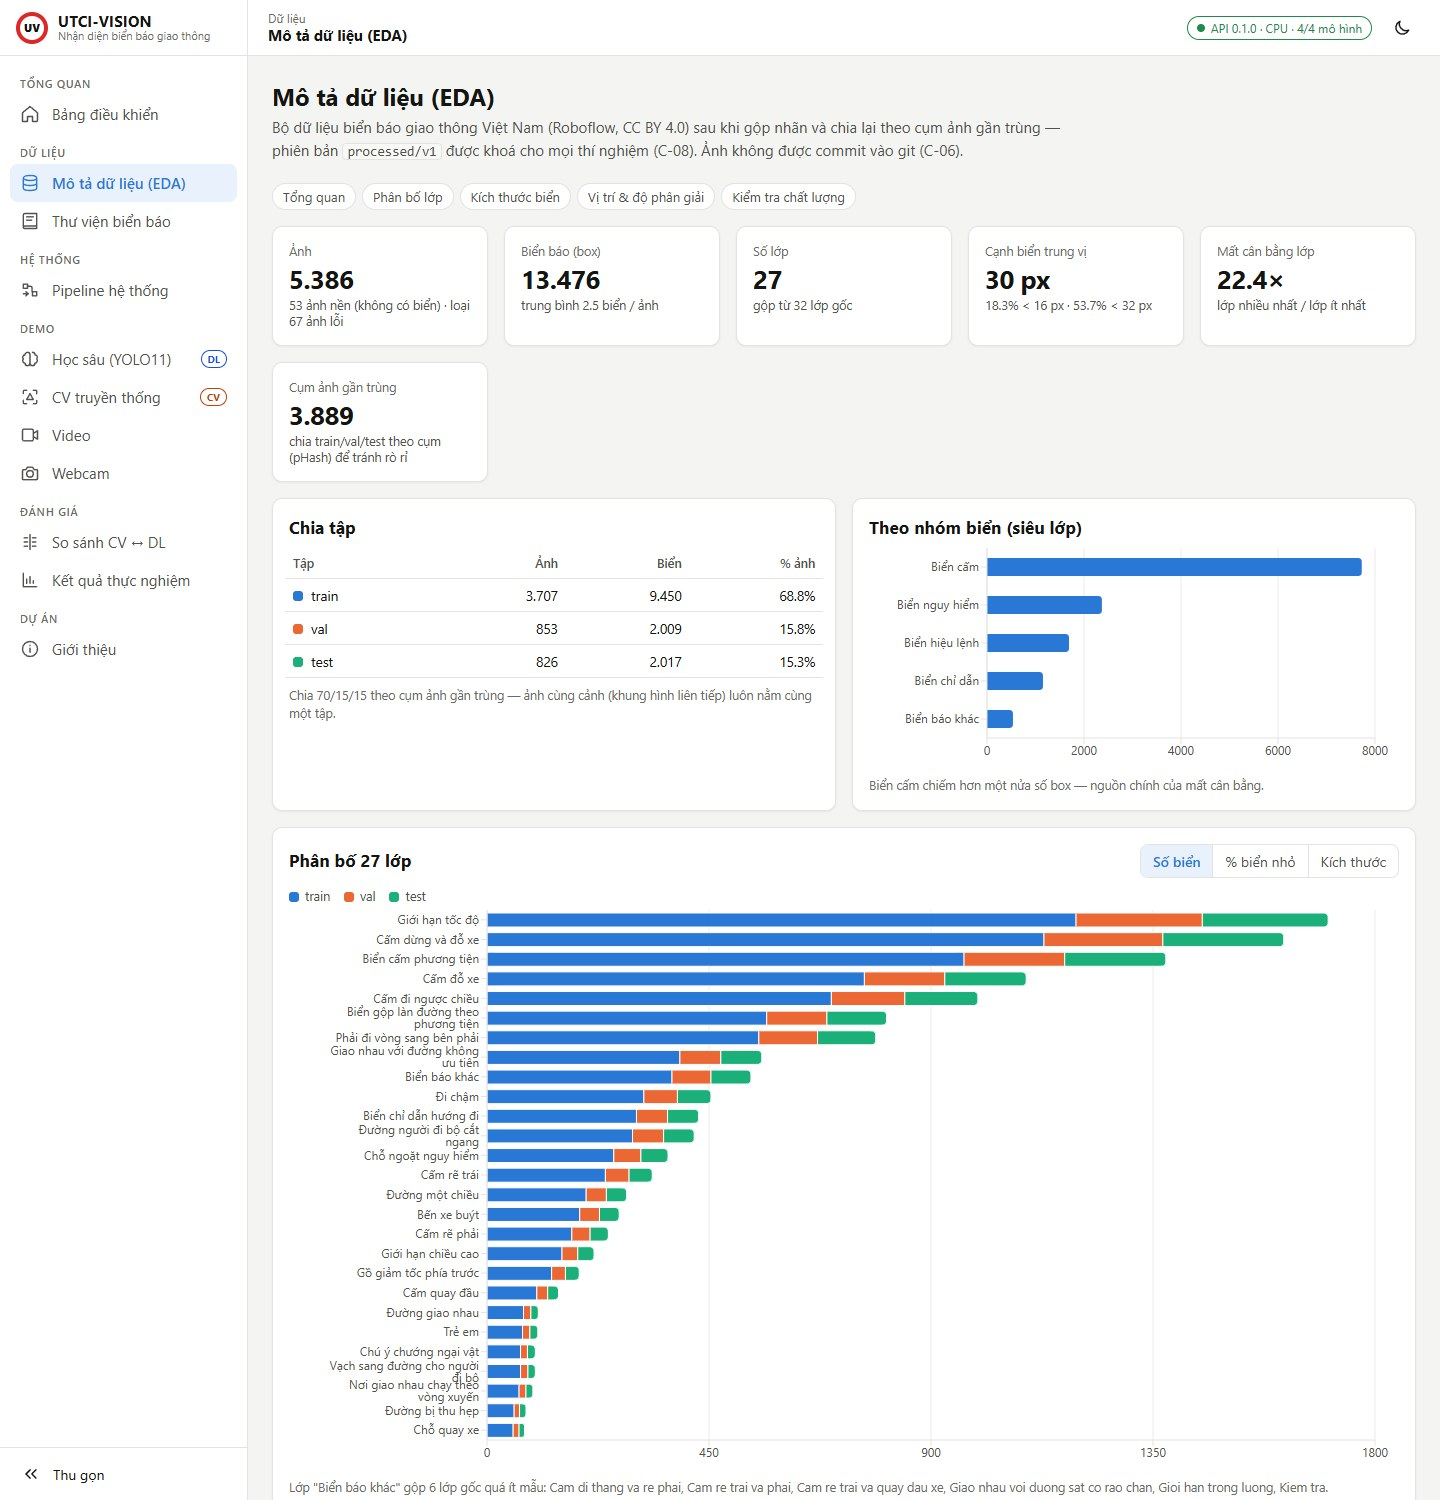
\includegraphics[width=.8\textwidth]{figures/web_eda.jpg}
\caption{Trang Mô tả dữ liệu của ứng dụng web}
\label{fig:web_eda}
\end{figure}

\begin{figure}[H]
\centering
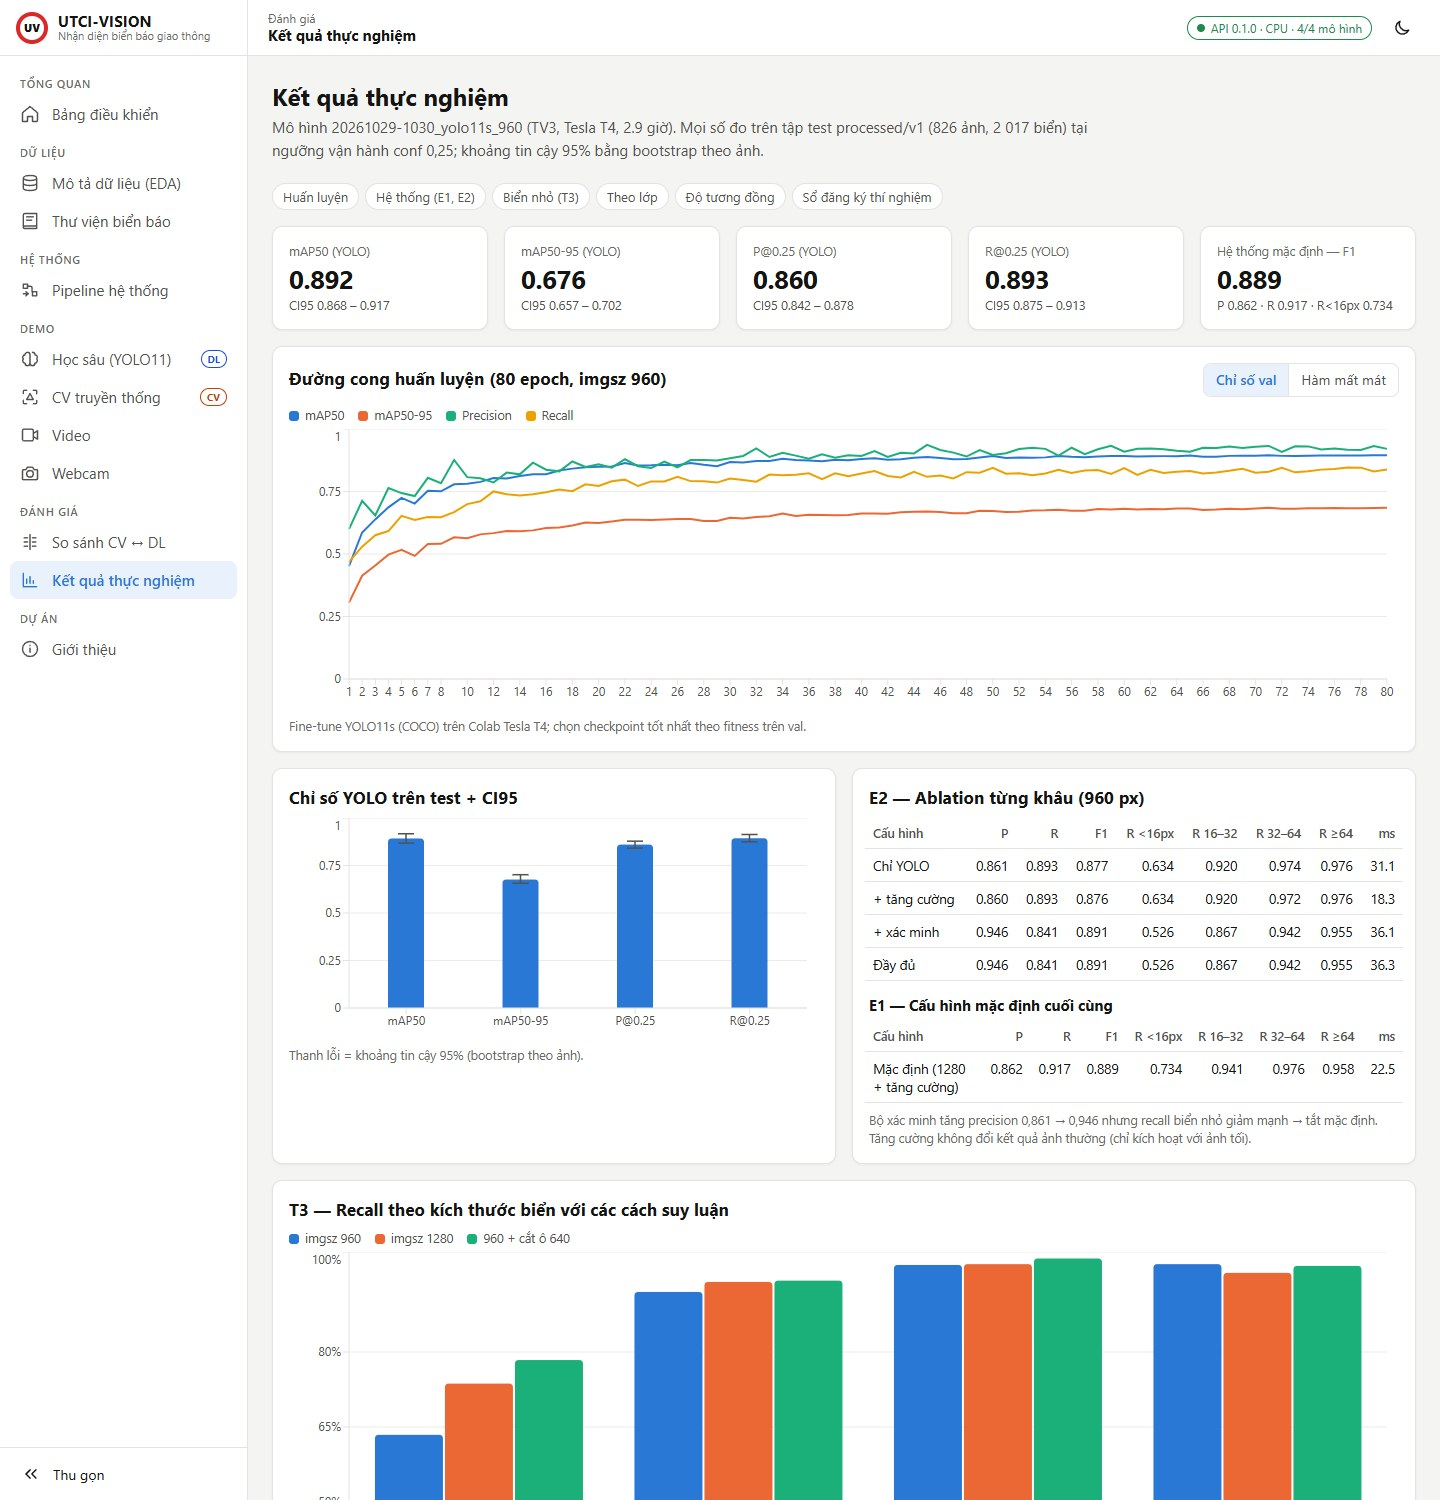
\includegraphics[width=.8\textwidth]{figures/web_results.jpg}
\caption{Trang Kết quả thực nghiệm của ứng dụng web}
\label{fig:web_results}
\end{figure}
